
\documentclass[a4paper,12pt]{article}
\date{}

%-----------------------------------------------------------------------------
% Language setting, set page size and margins
%-----------------------------------------------------------------------------
\usepackage[english]{babel}
\usepackage[a4paper,top=2.5cm,bottom=2.5cm,left=2cm,right=2cm,marginparwidth=1.75cm]{geometry}
\usepackage{setspace}
\setstretch{1.5}
%\onehalfspacing %interligne 1.5
%\doublespacing
%----------------------------------------------------------------------------

% Useful packages
\usepackage{amsmath}
\usepackage{amssymb}
\usepackage{graphicx}
\usepackage[hidelinks]{hyperref}
\usepackage{subfigure}
%\usepackage[colorlinks=true, allcolors=blue]{hyperref}

%\usepackage{fancyhdr}
%\fancyhead[C]{blabla}
%\fancyfoot[zone]{contenu} 

%----------------------------------------------------------------------------
% Packages: uncomment to debug
%----------------------------------------------------------------------------
%\usepackage{refcheck}
%\renewcommand{\labelitemi}{\textbullet}

%----------------------------------------------------------------------------
% Packages: bibliography
%----------------------------------------------------------------------------
%\usepackage[nottoc, notlof, notlot]{tocbibind}
\usepackage[authoryear,comma]{natbib}
%\usepackage[english]{babel}
\usepackage{authblk}

%----------------------------------------------------------------------------
% Acronyms
%----------------------------------------------------------------------------
\usepackage[acronyms]{glossaries}
\makeglossaries
%\newacronym{Identifiant unique}{Nom de l’acronyme}{Définition de l’acronyme}
\newacronym{kh}{KH}{Kelvin-Helhmoltz}

%----------------------------------------------------------------------------
% Page de garde
%----------------------------------------------------------------------------
\usepackage[utf8]{inputenc}
\usepackage[T1]{fontenc}
%\usepackage{fullpage}
\usepackage{eso-pic}
\newcommand{\HRule}{\rule{\linewidth}{0.5mm}}
\newcommand{\blap}[1]{\vbox to 0pt{#1\vss}}
\newcommand\AtUpperLeftCorner[3]{%
  \put(\LenToUnit{#1},\LenToUnit{\dimexpr\paperheight-#2}){\blap{#3}}%
}
\newcommand\AtUpperRightCorner[3]{%
  \put(\LenToUnit{\dimexpr\paperwidth-#1},\LenToUnit{\dimexpr\paperheight-#2}){\blap{\llap{#3}}}%
}

\title{ \Large{Rapport de Stage M2 SOAC-DC}}
\author{Marie Andrieux}
\makeatletter

%----------------------------------------------------------------------------
%----------------------------------------------------------------------------
%----------------------------------------------------------------------------
%                           BEGIN DOCUMENT
%----------------------------------------------------------------------------
%----------------------------------------------------------------------------
%----------------------------------------------------------------------------

\begin{document} 
%\maketitle
\thispagestyle{empty}

%----------------------------------------------------------------------------
% \ref with ( )
%----------------------------------------------------------------------------
\let\noparref\ref
\renewcommand{\ref}[1]{(\noparref{#1})}


%----------------------------------------------------------------------------
% Page de garde
%----------------------------------------------------------------------------
\begin{titlepage}
    \enlargethispage{2cm}
 
    \AddToShipoutPicture{
        \AtUpperLeftCorner{1.5cm}{2cm}{
\includegraphics[width=5cm]{figures/logoUPS.png}}
        \AtUpperLeftCorner{7.3cm}{1.3cm}{
\includegraphics[width=3.5cm]{figures/logoCNRS.png}}
        \AtUpperLeftCorner{11cm}{1cm}{
\includegraphics[width=4cm]{figures/logoLEGOS.png}}
        \AtUpperRightCorner{1.5cm}{2cm}{
\includegraphics[width=4cm]{figures/logoLA.jpg}}
        }
 
    \begin{center}
        \vspace*{5cm}
        \textsc{\@title} \\
        \vspace*{0.5cm}
        \textsc{\Large Université Paul Sabatier} \\
        \vspace*{2cm}
        \large{\bf Influence de la diffusion moléculaire sur le mélange de traceurs passifs}
        \HRule
        \vspace*{0.5cm}
        \large{\@author} \\
        \vspace{1cm}
        \small{Tuteurs : Yves Morel (Legos), Francis Auclair (Laero) et Cyril Nguyen (Laero)}
        
    \end{center}
 
    \vspace*{2.5cm}
 
    \begin{center}
        \makebox[\textwidth]{\includegraphics[width=\paperwidth]{figures/Imageinstabilité.jpg}}
    
    \vspace{0.3cm}
    \small{\bf Février - Août 2022}
    \end{center}
 
\end{titlepage}
\ClearShipoutPicture

\newpage
 
%----------------------------------------------------------------------------
% Page numbering
%----------------------------------------------------------------------------
\renewcommand{\thepage}{\arabic{page}}
\setcounter{page}{1}

%----------------------------------------------------------------------------
%%  ABSTRACT
%----------------------------------------------------------------------------
\newpage
\begin{abstract}
25 à 30 pages maximum dont le contenu indicatif est le suivant : 1 résumé, 1 table des matières, 1 liste des acronymes si nécessaire, 1 introduction (posant la problématique, restituant les questions abordées dans leur contexte scientifique ou industriel, et présentant la démarche utilisée/suivie pour aborder cette thématique), 1 description de la méthodologie, 1 présentation des résultats ou des cas d’étude, 1 discussion, 1 conclusion avec des perspectives, 1 conclusion personnelle d’une demi-page précisant les
apports du stage (pour le rapporteur de l'université, pas nécessairement dans le rapport à l'encadrant), bibliographie.  Le rapport peut être rédigé en anglais ou en français.
- Possibilité de mettre des annexes (utiles pour l’équipe d’accueil/l’entreprise) qui ne seront pas évaluées et dont la lecture ne doit pas être indispensable à la compréhension du rapport. - Format impératif du rapport : police caractères taille 12, marges 2,5 cm, interligne 1.5.
\end{abstract}

%----------------------------------------------------------------------------
%%  TABLE DES MATIERES
%----------------------------------------------------------------------------
\newpage
\renewcommand*\contentsname{Table des Matières}
\tableofcontents

%\newpage
%\printglossary[type=\acronymtype]

%----------------------------------------------------------------------------
%%  ACRONYMES
%----------------------------------------------------------------------------
\newpage
Liste des acronymes \\
Remerciements\\

%----------------------------------------------------------------------------
%%  INTRODUCTION
%----------------------------------------------------------------------------
\newpage
\section{Introduction}

    \textbf{\textit{Le mélange dans l'océan}} \\
    %Contexte, c'est quoi le mélange, comment il agit dans l'océan, quel est son impact ? \\
    %Le mélange est l'action d'homogénisation d'un volume fluide. Dans le cas de l'océan, il correspond à la redistribution de propriétés de masse d'eau comme la chaleur, la salinité, les espèces chimiques et biologiques. 
    À l'échelle globale, l'océan a une stratification stable, mais si on s'intéresse aux petites échelles, le mélange diapycnal devient important. Les processus de mélange sont importants au niveau des bords des océans (tension du vent, frottement de fond) mais aussi dans le $~95\%$ restant de la colonne d'eau. Ce mélange concerne aussi bien les traceurs passifs, actifs et réactifs. Les traceurs passifs n'ont pas d'effet direct sur la dynamique et pas d'activité biogéochimique à court terme. C'est le cas de certaines espèces à faible concentration ou à flottabilité neutre \citep{warhaft_passive_2000,canuto_vertical_2011}. Ceux-ci comprennent, dans l'océan, les nutriments, les espèces biologiques microscopiques \citep{vaquer-sunyer_thresholds_2008,brierley_impacts_2009}, et certains éléments traces/radioéléments (\cite{broecker_distribution_nodate} 1970 1976). Les traceurs actifs, comme la densité, la température et la salinité, ont une influence sur la dynamique. Les traceurs réactifs sont des espèces biologiques et/ou chimiques capables de réagir avec certaines espèces environnantes. C'est le cas, par exemple, des espèces participant aux réactions biogéochimiques comme les phytoplanctons, les composants azotés, les phosphates et les éléments carbonés. 
    \\
    Loin des bords dans l'océan, le mélange vertical peut être déclenché par des instabilités dynamiques de cisaillement telles que les instabilités de Kelvin-Helmholtz (\cite{smyth_ocean_2012}). Ces instabilités ont été largement étudiées depuis leur théorisation par Lord Kelvin, en 1868, et Hermann Von Helmholtz, en 1871. À la fois avec des études expérimentales en laboratoire (Thorpe 1973, \citet{caulfield_secondary_1996,patterson_time-dependent_2006}, avec des simulations numériques (\cite{klaassen_role_1989}, \cite{caulfield_three_1994}, Scinocca 1995, \cite{alexakis_stratified_2009}, \cite{carpenter_identifying_2010}, Balmforth & Lawrence 2010, \cite{mashayek_shear-induced_2013}, \cite{mashayek_zoo_2012}). Les instabilités de KH sont également observées dans l'océan dans des zones de forts cisaillements : le long des thermoclines océaniques (\cite{woods_wave-induced_1968}, Marmorino 1987), pendant les phases de marée descendante près des monts sous-marins (\cite{van_haren_deep-ocean_2010}) et aussi à la limite de la couche de surface de mélange qui a tendance à s'abaisser avec ces instabilités de cisaillements (\cite{lincoln_surface_2016}). Dans les estuaires, on retrouve ces instabilités au niveau des interfaces (Geyer & Smith 1987,  \cite{geyer_mixing_2010}) qui peuvent être riches en espèces chimiques et nutriment à cause des apports fluviaux. 
    \\
    Dans l'océan, les études de l'effet des instabilités KH ont été motivées par l'importance probable des processus de mélange sur la stratification globale et donc la circulation à grande échelle (par exemple \cite{wunsch_v_2004}), et par analogie, ils sont également importants pour la distribution verticale des espèces chimiques et biologiques. Compte tenu de l'impact du mélange turbulent sur les distributions macroscopiques/grandes échelles de traceurs, il est important de bien comprendre ces processus qui sont la clé de notre capacité à modéliser et prévoir l’évolution des ressources, la qualité de l'eau, le développement et la dispersion de certains polluants, la production primaire (plancton) et l’évolution des ressources halieutiques dans l'océan qui représentent des problèmes de société importants pour une gestion et une exploitation durable de l’environnement. 
    \\
    Les modèles océaniques sont généralement établis pour résoudre l'échelle régionale ou globale des bassins dans une démarche de compréhension de la circulation et du transport des traceurs. Pour éviter les coûts de calculs aberrants, les résolutions horizontales sont de l'ordre du kilomètre à plusieurs kilomètres et la résolution verticale d'une dizaine de mètres à la centaine de mètres. Mais ces résolutions excluent les processus petites échelles comme la dissipation turbulente et le mélange irréversible qui sont pourtant essentiels pour établir l'intensité de la circulation océanique et la distribution des propriétés des masses d'eau (John Toole 1998). Des paramétrisations de processus sous-maille sont donc mis en place tels que les modèles KTE utilisent une équation d'évolution et de dissipation de l'énergie cinétique turbulente sensible aux forçages turbulents (cisaillement, convection, tension du vent, frottement de fond). Mais il existe une grande variété de paramétrisation.\\
    \newline
    \textbf{\textit{De l'instabilité de Kelvin-Helmholtz vers la cascade turbulente}} \\
    Les instabilités de KH sont des sources de cascade turbulente, et donc potentiellement de mélange efficace, c'est-à-dire de mélange avec un impact sur les profils macroscopique. Dans cette étude, on a choisi ces instabilités pour créer du mélange turbulent, mais les résultats pourraient potentiellement s'appliquer à toutes autres sources d'instabilité. Les instabilités KH se produisent à la frontière entre deux fluides ayant des vitesses différentes. Cependant, la stratification de la colonne d'eau a tendance à stabiliser l'écoulement. Une condition nécessaire pour avoir une instabilité de KH est d'avoir un nombre de Richardson intérieur à 0.25 (\cite{peltier_m_2003} ??? a vérif plutot article de 1994), sachant qu'il représente un rapport entre la fréquence de Brunt-Vaisala ($\approx$stratification) et le carré du cisaillement de vitesse horizontale : \\
    \begin{equation}
        Ri = -\frac{g \dfrac{\partial\rho}{\partial z}}{\rho_0 (\dfrac{\partial u}{\partial z})^2}
        \label{Ri}
    \end{equation}
    \\
    L'instabilité KH est caractérisée par la formation d'un vortex 2D, appelé "cat eyes" dans la littérature. La longueur d'onde et de ce vortex peut être prédit avec la théorie de Taylor-Gloldstein qui découle d'une dérivation des équations d'Euler avec une approximation de Boussinesq. Une résolution numérique de valeurs propres (taux de croissance et longueur d'onde) est proposé par Hazel, 1971, pour obtenir la longueur d'onde la plus instable. Une fois le vortex saturé en énergie, une cascade turbulente se met en place pour transférer cette énergie des grandes échelles vers les petites échelles (Peltier et al. (1978), Davis \& Peltier (1979), \cite{klaassen_onset_1985} \cite{klaassen_role_1989}). Des instabilités transverses (3D) apparaissent ensuite et la diffusion moléculaire commence à être efficace à cause des forts gradients locaux formés par l'étirement et l'advection dans la couche de cisaillement (\cite{caulfield_three_1994}).  \\
    \newline
    \textbf{\textit{Problématique}} \\
    Les paramétrisations de processus turbulents sont des astuces pour gagner en temps de calcul et par conséquent impliquent des hypothèses et des simplifications des processus. Souvent, les coefficients de diffusion des traceurs sont choisis de manière ad hoc/empirique avec une valeur constante autour de $10^{-4}$ $m^2.s^{-1}$ pour tous les traceurs. Mais ces paramétrisations peuvent être une grande source d'incertitudes dans les sorties des modèles, car elles ne représentent pas exactement les processus fines-échelles. 
    \\
    L'étude théorique et numérique de \cite{penney_diapycnal_2020} avec des traceurs passifs a montré qu’il existe des contraintes fortes sur l’évolution macroscopique des traceurs : le mélange engendre une simplification des interdépendances entre traceurs, qui deviennent linéaires. Ils ont montré que cela contraint tous les traceurs à avoir une diffusivité turbulente macroscopique égale et à pouvoir être tous entièrement déterminés à partir de la connaissance de l'évolution d’un seul traceur. Ces expériences mettent en évidence comment des propriétés à échelle moléculaire peuvent avoir des répercussions majeures à échelle macroscopique. Cependant, ces résultats ont été établis dans le cas précis d’égalité des diffusivités moléculaires pour tous les traceurs. Le but de ce stage est d'étudier les effets d’une diffusion moléculaire différente entre traceurs passifs et densité, et de comprendre comment le lien entre l'évolution macroscopique du traceur et de la densité évolue.  
    \\
    Pour ce stage, l'étude de l'impact du mélange moléculaire sur les profils macroscopiques passe par une modélisation numérique fine échelle d'une colonne d'eau soumise à un cisaillement de vitesse horizontale. Ensuite, des analyses physiques ont été mises en place pour comprendre, dans un premier temps, si la cascade turbulente créer du mélange efficace, puis, dans un second temps, pour analyser l'impacte de ce mélange à l'échelle macroscopique. Notamment pour mettre en évidence les différences de comportement avec l'étude de \cite{penney_diapycnal_2020}.
    \\
    Le modèle CROCO, utilisé pour les simulations, et les formalismes employés pour les analyses physiques sont présentés dans la partie Méthode. La seconde partie se concentre sur les détails de la configuration numérique mise en place pendant le stage, et les simulations effectuées. Les résultats sont séparés en trois parties. Pour commencer, les résultats issus des simulations ou le coefficient de la densité varie, ensuite les résultats issus des simulations ou le coefficient de diffusion du traceur passif varie, puis les résultats de l'analyse macroscopiques. Dans la partie suivante, les résultats seront discutés, et on terminera par une conclusion.

%----------------------------------------------------------------------------
%%  METHODE
%----------------------------------------------------------------------------
\newpage
\section{Méthode}

%--Modèle Croco--------------------------------------------------------------
    \subsection{Le modèle CROCO-NBQ}
    
    Les simulations présentées ici ont été réalisées avec le modèle CROCO (Coastal and Regional Ocean Community) en version non-Boussinesq et non-hydrostatique.
    CROCO est un modèle dédié à l'océan, notamment à la modélisation de l'échelle régionale, issu du code numérique ROMS (Regional Ocean Modeling System) auquel a été ajouté les effets compressibles et non-hydrostatiques \citep{auclair_non-hydrostatic_2018}. \\
    \newline
    NBQ (Non-Boussinesq) signifie qu'on ne fait pas l'approximation de Boussinesq qui est une approximation classique en physique de l'océan. Elle consiste à supposer que la densité de l'eau de mer varie peu dans l'espace et dans le temps autour d'une valeur moyenne $\rho(x,y,z,t)=\rho_{0}+\rho'(x,y,z,t)$. Cette hypothèse permet de négliger les variations de densité dans les équations de Navier-Stokes à l'exception du terme de gravité. Or dans notre étude, nous avons besoin de ces termes de variation de densité puisqu'on étudie le mélange diapycnal. \\
    \newline
    L'approximation hydrostatique est aussi une approximation classique en physique de l'océan, car elle est basée sur le fait que les longueurs horizontales des bassins sont très grandes devant les longueurs verticales. Les termes d'accélérations verticales sont donc négligés, ce qui mène à l'équilibre hydrostatique. Or ici, nous avons besoin de cette accélération verticale pour créer des instabilités. Cependant, imposer des conditions non-hydrostatiques dans un modèle est complexe. En effet, les anomalies de pression totale sont rayonnées par des ondes acoustiques beaucoup plus rapides dans l'océan que n'importe quel courant et n'importe quel type d'ondes de gravité et leur simulation explicite est plus gourmande en ressources informatiques. En conséquence, les modélisateurs ont deux choix pour mettre en œuvre un algorithme non hydrostatique : soit ils filtrent les ondes acoustiques (mais ils doivent résoudre un système de Poisson 3D elliptique pour récupérer la pression totale), soit ils simulent explicitement les ondes acoustiques (mais ils doivent s'appuyer sur un pas de temps numérique très efficace).
    CROCO opte pour la deuxième solution et propose un fractionnement temporel avec d'une part les processus "lent" (advection, diffusion, transfert) et d'autre part les processus "rapides", non-Boussinesq (ondes acoustiques, surface libre). Les vitesses caractéristiques maximales peuvent donner un ordre de grandeur pour les échelles de temps les plus restrictives pour chacun de ces processus. La dynamique "lente" est associé au champ de vitesse explicite (ici, $U=1 m/s$), alors que la vitesse des ondes de surfaces est environ $c_g=50 m/s$ et les ondes acoustiques se propagent à $c_s=1500 m/s$ dans l'eau. Cette dernière vitesse impliquerait un coût numérique trop important à cause des conditions CFL ($\frac{\Delta x}{\Delta t}>c$). Or dans notre étude, les ondes acoustiques ne sont pas étudiées, elles doivent seulement parcourir tout le domaine avant les autres processus, ce qui autorise une réduction de leur vitesse à 200 m/s ($=4*c_g$). Dans un premier temps, la distance entre l'instabilité et la surface libre est considéré comme suffisante pour qu'elles n'aient pas d'interaction, ce qui permet de réduire encore plus la vitesse acoustique (mais ne pas résoudre correctement la surface libre en contrepartie.)\\

%--Analyse physique----------------------------------------------------------------
    \subsection{Analyse physique}
    
        \subsubsection{Diagramme de dispersion}
        
        Pour suivre le mélange diapycnal, les propriétés des particules fluides peuvent être représentées dans un espace 2D, avec, en coordonnées, la concentration en traceur et la densité. 
        Ce diagramme de dispersion met en évidence les changements de caractéristiques de particules. En effet, une particule fluide reste à la même position dans ce diagramme quelque soit son déplacement ou sa déformation géométrique dans l'espace physique. En revanche, si les propriétés sont modifiées par un mélange irréversible dans l'espace physique, la distribution des particules fluides changera dans ce diagramme de dispersion. Par exemple, sur la figure \ref{Fig8}, l'advection ne modifie pas le nuage de point, mais peut rapprocher des particules fluides avec des propriétés différentes, comme les quatre particules vertes. Le mélange homogénéise les caractéristiques densité-traceur des parcelles à l'intérieur d'une cellule dont la taille est déterminée par le coefficient de diffusion. Les caractéristiques densité-traceur résultants de cette cellule sont alors les valeurs moyennes des propriétés initiales, pondérées par leur rapport volumétrique (par exemple le point rouge). Cela implique que le nuage de points, après advection et mélange, sera contenu dans l'enveloppe convexe de la distribution initiale (région à l'intérieur de la courbe en pointillés rouges). \\
        \begin{figure}[!h]
            \centering
            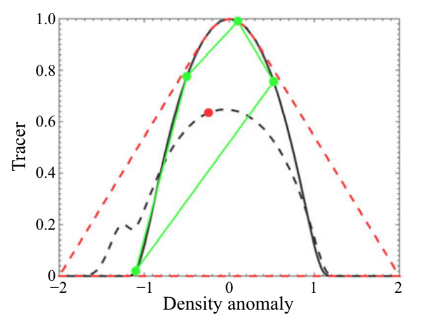
\includegraphics{figures/fig8_Jared.PNG}
            \caption{\textit{Diagramme de dispersion schématique (traceur-densité) issus de
            \cite{penney_diapycnal_2020}.}}
            \label{Fig8}
        \end{figure}
        \newline
        Des diagrammes similaires sont souvent utilisés pour caractériser le mélange dans les flux géophysiques, tels que les diagrammes température-salinité utilisés pour quantifier le mélange de grandes masses d'eau dans l'océan (par exemple \citep{tomczak_multi-parameter_1981}) ; les courbes de mélange traceur-salinité dans une embouchure, utilisées pour déterminer si un estuaire peut agir comme source ou puits d'un traceur donné (par exemple, \citep{loder_dynamics_1981} et \cite{officer_dynamics_1981}); ou des diagrammes de traceurs-traceurs utilisés pour examiner les relations compactes entre différents traceurs atmosphériques (par exemple, \cite{tilmes_development_2006} et \cite{plumb_tracer_2007}). Les diagrammes de dispersion sont donc pratiques pour l'analyse présentée ici, car ils permettent l'identification directe du mélange de traceur dans des nouvelles gammes de densités
        %transport de traceurs diapycnal 
        qui doit être indiqué par la génération de nouveaux points dans l'espace densité-traceur.\\
        %\newline
        Pour mieux représenter la distribution en densité et traceur, chaque point dans cet espace est associé à un "poids" qui est une formulation discrète de la fonction de probabilité densité-traceur présentée dans l'annexe D de \cite{plumb_tracer_2007}. Le poids de chaque point quantifie sa concentration en densité ou traceur, il est représenté par l'échelle de couleur sur les figures. \\
        \newline
        \cite{plumb_tracer_2007}, \cite{lauritzen_evaluating_2012} ont déjà utilisé cette méthode pour déterminer si le mélange dans les modèles numériques est physique. \cite{penney_diapycnal_2020} ont montré que si l'évolution de la densité et du traceur est gouvernée par une équation d'advection-diffusion et que les coefficients de diffusion moléculaire de densité et de traceur passif sont égaux, il existe une contrainte sur l'évolution de ce diagramme. Dans ces conditions, les particules restent confinées dans l'enveloppe convexe du pas de temps précédent (Figure \noparref{Fig8}) ce qui induit une diminution de cette enveloppe au cours du temps jusqu'à une convergence de la relation traceur densité pour atteindre une forme linéaire par morceaux.
    
    
        \subsubsection{Réarrangement isopycnal}
        
        Le réarrangement isopycnal est un formalisme pour visualiser l'évolution macroscopique de l'instabilité en trouvant, de manière conservative, un profil vertical 1D à partir du domaine 3D. Il a été introduit par \citep{nakamura_two-dimensional_1996} et \citep*{winters_diascalar_1996} pour des écoulements spatialement inhomogènes où les traceurs sont advectés et diffusés. C'est un changement des coordonnées cartésiennes vers des coordonnées basées sur l'organisation géométrique d'un traceur (ici la densité). Les isosurfaces de densité sont indexées par leur volume pour être réorganisées de manière stable. Autrement dit, les éléments fluides, chacun avec un volume infinitésimal spécifié, sont classés par leur densité, donnant la densité en fonction du volume cumulé, puis le volume est converti en coordonnée verticale $z_*$ en divisant par la surface horizontale du fluide domaine. Ainsi, on réarrange les parcelles fluides en changeant leur forme, mais en conservant leur volume (Figure \ref{rea_isop}-a,b). Les nouvelles distributions en traceur exprimées en fonction ce ces nouvelles coordonnées seront notées avec une étoile ($\rho_*$ et $\phi_*$).
        \begin{figure}[!h]
	    \centering		
		    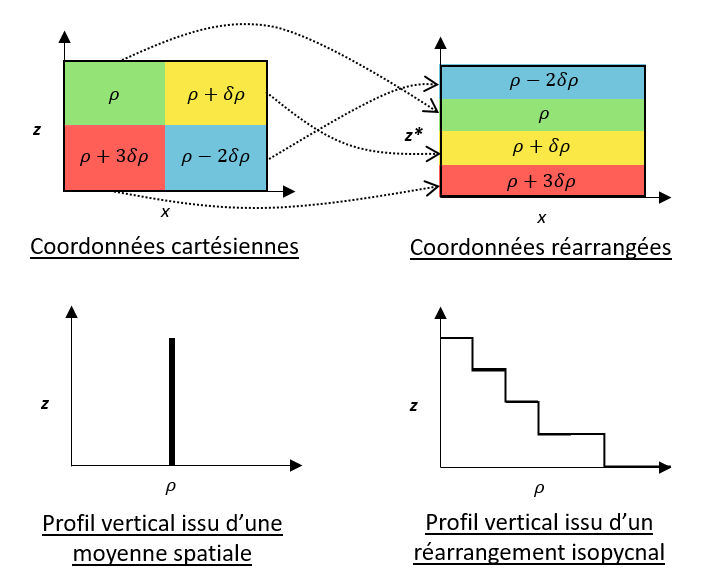
\includegraphics[width=0.85\linewidth]{figures/rearrangementisop.png}
            \caption{\textit{Schéma illustratif du réarrangement isopycnal. (a) distribution en coordonnées cartésiennes, (b) même distribution en coordonnées $z*$, (c) profil vertical issu d'une moyenne spatial, (d) profil vertical issu du réarrangement isopycnal.}}
	        \label{rea_isop}
        \end{figure}
        Ce réarrangement isopycnal est en faite une représentation macroscopique des processus diffusif. Il a l'avantage d'être conservatif, c'est-à-dire de ne pas modifier les propriétés des particules, le terme de réarrangement adiabatiques est souvent utilisé dans la littérature. C'est le seul moyen connu d'obtenir un profil macroscopique sans rajouter de processus non conservatif (diabatique) contrairement à une moyenne spatiale qui, par définition, homogénéise les propriétés sur un espace donné (Figure \ref{rea_isop}-c,d). \\
        Le profil obtenu issu du réarrangement de la densité est le profil de plus basse énergie potentielle et il ne varie au cours du temps qu'avec des processus non conservatif, i.e avec le mélange (\cite*{winters_diascalar_1996}.
        
        \subsubsection{Diffusion effective}
        
        La diffusion effective est la diffusion efficace à l'échelle macroscopique. Comme le profil macroscopique (issus du réarrangement isopycnal) ne varie qu'avec des processus non conservatif, son évolution peut être approximée sous la forme d'une simple équation de diffusion (\citep{penney_diapycnal_2020-1}) : 
        \begin{equation}
            \label{rho*}
            \frac{\partial\rho_*}{\partial t}=\frac{\partial}{\partial z_*}(K_{\rho}\frac{\partial\rho_*}{\partial z_*})
        \end{equation}
        Avec $K_{\rho}$ la diffusion effective, seule inconnue de cette équation, l'évolution de $\rho_*$ nous est donnée par le réarrangement isopycnal de la sortie de la simulation. La diffusion effective peut donc être extraite de cette équation :
        \begin{equation}
            \label{Keff}
            \frac{K_{\rho}}{\kappa_{\rho}}=\frac{\langle\vert\Delta\rho\vert^2\rangle_{z_*}}{(\dfrac{\partial\rho_*}{\partial z_*})^2}
        \end{equation}
        Une fois cette diffusion effective calculée, on peut l'appliquer aux profils initiaux de la densité à travers une simple équation de diffusion macroscopique. Le profil final obtenu doit être le même que le profil final de la densité réarrangé. C'est donc une manière d'obtenir un coefficient de diffusion macroscopique utilisable dans des paramétrisations sous-maille des processus non conservatif. \cite{penney_diapycnal_2020} ont monté que si le coefficient de diffusion moléculaire d'un traceur passif est le même que celui de la densité, alors un traceur virtuel calculé avec cette même diffusion effective peut prédire le profil final du traceur. Rigoureusement, l'évolution du traceur réarrangé s'écrit : 
        \begin{equation}
           \frac{\partial\phi^*}{\partial t} = \frac{\partial}{\partial z^*} (\frac{\kappa_{\phi}}{\kappa_{\rho}}K_{\rho}\frac{\partial\phi^*}{\partial z^*}) + \frac{\partial}{\partial z^*} ((\frac{\partial\rho^*}{\partial z^*})^{-1} \langle\kappa_{\phi}\nabla\phi'\cdot \nabla\rho - \kappa_{\rho}\phi'\nabla^2\rho\rangle_{z^*})
           \label{phi*}
        \end{equation}
        Mais le coefficient de diffusion effectif peut être appliqué à un traceur virtuel, pour lequel seul le premier terme, associé au flux diffusif du traceur à travers les isopycnes, est considéré (le second terme, plus compliqué, associé au mouvement des isopycnes par rapport au fluide est négligé). L'évolution du traceur virtuel s'écrit donc :
        \begin{equation}
            \frac{\partial\phi_v}{\partial t} = \frac{\partial}{\partial z^*} (\frac{\kappa_{\phi}}{\kappa_{\rho}}K_{\rho}\frac{\partial\phi_v}{\partial z^*})
        \end{equation}
        
%----------------------------------------------------------------------------
%%  CONFIGURATION NUMÉRIQUE
%----------------------------------------------------------------------------        
\section{Configuration numérique}
    
%---Conditions initiales------------------------------------------------------    
    \subsection{Conditions initiales}
    
    Les équations sont toutes adimentionalisées par des échelles typiques des instabilités KH.  Par conséquent, les valeurs présentées sur les figures sont également sans dimensions. Les variables dimensionnelles sont notées avec des tildes. 
    \begin{center}
       $x=\Tilde{x}/h$  \hspace{1cm}  $y=\Tilde{y}/h$  \hspace{1cm}   $z=(\Tilde{z}-z_0)/h$   \hspace{1cm}    $t=\Tilde{t}U_0/h$    \hspace{1cm}  $u=\Tilde{u}/U_{0}$    \hspace{1cm}   $\rho =( \Tilde{\rho}-\rho_0)/\Delta\rho$   \hspace{1cm}     $\phi=\title{\phi}/\Delta\phi$ \\ 
    \end{center}
    Avec $h$ la hauteur de la couche du cisaillement, $z_0$ le milieu du domaine vertical (également centre de la couche de cisaillement), $U_0$ la moitié de la variation de vitesse initiale sur le domaine, $\rho_0$ la densité médiane sur la distribution initiale de densité, $\Delta\rho$ la moitié de la variation de densité initiale sur tout le domaine et $\Delta\phi$ la concentration initiale maximale du traceur.\\
    \newline    
    \textbf{Densité} \\
    La distribution initiale de densité est linéaire, ainsi chaque particule fluide a une position unique sur le diagramme de dispersion initial :
    \begin{equation}
    \label{rho_ini}
        \rho(x,y,z,t=0)=-z\Delta\rho
    \end{equation}
    Le choix de la stratification, $\Delta\rho$, affecte le nombre de Richardson. Dans cette étude $\Delta\rho=1.2$ est assez faible pour avoir un $Ri=4.5\ 10^{-3}<< 1/4$. Cependant, si la stratification venait à augmenter, le nombre de Richardson dépasserait difficilement la valeur de 1/4 avec une telle configuration (Figure \noparref{TG_deltarho}). Il en est de même pour la longueur d'onde la plus instable,  d'après la théorie de Taylor-Golstein, elle ne varie que très peu avec $\Delta\rho$ dans cette étude. \\
    \begin{figure}[!h]
	\centering		
		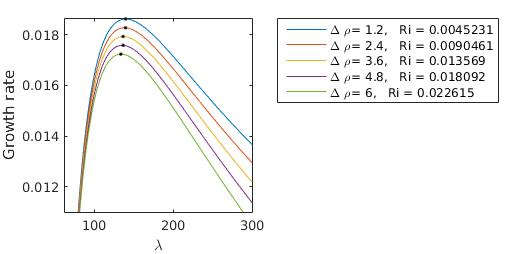
\includegraphics[width=0.9\linewidth]{figures/TG_delatrho_2.jpg}
\caption[Taylor-Goldstein]{\textit{Prédiction du taux de croissance en fonction de la longueur d'onde d'après la théorie de Taylor-Goldstein pour plusieurs gammes de stratifications}}
	\label{TG_deltarho}
\end{figure}
    \newline
    \textbf{Vitesse} \\
    Le champ de vitesse initiale est : 
    \begin{subequation}
    \begin{align}
        \displaystyle
            \label{u_ini}
            & u(x,y,z,t=0)=U(z)+u'(x,y,z) \\
            \label{v_ini}
            & v(x,y,z,t=0)=v'(x,y,z) \\
            \label{w_ini}
            & w(x,y,z,t=0)=w'(x,y,z)
    \end{align}
    \end{subequation}
    $U(z)$ est le cisaillement vertical de vitesse initial. Il est sous la forme d'une tangente hyperbolique centrée,
    \begin{equation}
        \label{u0_ini}
        U(z)=-tanh(z)
    \end{equation}
    ainsi la couche supérieure va vers la gauche et la couche inférieure vers la droite avec la même vitesse. $u', v'$ et $w'$ sont les petites perturbations nécessaires pour enclencher l'instabilité. Leur forme est choisie pour que le champ de vitesse initiale soit non divergent.
    \begin{subequation}
        \begin{align}
        \displaystyle
            \label{u'_ini}
            & u'(x,y,z)=\epsilon f'(z)\sin{(\frac{2\pi n_x}{L_x}x)}(1+\epsilon_{3D}\sin{(\frac{2\pi n_y}{L_y}y)}) \\
            \label{v'_ini}
            & v'(x,y,z)=0 \\
            \label{w'_ini}
            & w'(x,y,z)=-\epsilon f(z)\frac{2\pi n_x}{L_x}\cos{(\frac{2\pi n_x}{L_x}x)}(1+\epsilon_{3D}\sin{(\frac{2\pi n_y}{L_y}y)})
        \end{align}
    \end{subequation}
    La fonction $f(z)$ localise la perturbation initiale dans la région du cisaillement : 
    \begin{equation}
        f(z)=1-tanh^2(z)
    \end{equation}
    %\[f(z)=1-tanh^2(\frac{z}{\alpha})\]
    %Avec $\alpha=4.29$ et $\epsilon=0.01$
    Avec $\epsilon=0.01$ pour un paramètre sans dimension qui définit l'amplitude de la perturbation dans le sens du courant et $\epsilon_{3D}=0.2$ l'amplitude transverse. $n_x$ et $n_y$ définissent respectivement les longueurs d'ondes dans la direction x et y. \\
    \newline
    \textbf{Traceur passif} \\
    Le traceur passif est concentré dans la couche de cisaillement avec une forme :
    \begin{equation}
    \label{phi_ini}
        \phi(x,y,z,t=0)= a\Delta\phi sech^2(az-b)
    \end{equation}
    Avec les constantes $a=1$, qui contrôle l'épaisseur de la couche initiale, et $b=0$, qui contrôle la position de la couche de traceur par rapport au milieu vertical du domaine. 
    
%---Paramètres numériques-----------------------------------------------------    
    \subsection{Paramètres numériques}
    
    
    Toutes les simulations présentées ici ont les mêmes conditions initiales sur la structure de la densité, du traceur et du champ de vitesse. Les nombres sans dimensions sont également constants, Ri=0.0045 et Re=2000. La longueur d'onde sans dimension la plus instable prévu par la théorie de Taylor-Godstein dans ces conditions est $\lambda_{KH}=14.0$. La longueur du domaine est choisie telle que $L_x\approx \lambda_{KH}$ pour n'avoir qu'un seul vortex qui se forme. Les nombres de points de grille ($N_x$, $N_y$ et $N_z$ respectivement dans les directions x, y et z) sont choisis pour avoir une résolution sans dimension isotrope : $\Delta x=\Delta y=\Delta z=0.055$. Alors que les simulations numériques des instabilités KH sont souvent considérées dans un domaine periodique avec une surface et un fond rigide à glissement, ici la surface est libre et le fond est rigide et immobile. Les conditions de bord latérales sont périodiques à la fois dans la direction $x$ et dans la direction $y$. 
    
%---Tests numériques----------------------------------------------------------    
    \subsection{Tests numériques}
    
    La configuration numérique à d'abord été testée avec des cas simplifiés en 2D afin d'optimiser le temps de calcul. Des tests de réduction de la vitesse acoustiques ont été effectués pour évaluer jusqu'à quel point elle peut être réduite sans impacter la dynamique à laquelle on s'intéresse. Les simulations ont été comparées à une simulation de référence pour laquelle la vitesse acoustique est de $c_s=200 m/s$. Il a été conclu que la vitesse acoustique minimale utilisable dans cette configuration est $c_s=10 m/s$, pour laquelle on gagne un facteur 100 sur le coût de calcul par rapport à une vitesse acoustique réelle de $c_s= 1500 m/s$.
   
%---Liste des simulations----------------------------------------------------------     
    \subsection{Liste des simulations}
    Afin de faire varier le rapport entre les diffusions moléculaires de la densité et du traceur, 5 simulations ont été évaluées. La première (cas 1) est un cas de référence avec des coefficients de diffusion similaire pour le traceur et la densité, on attend donc des résultats similaires à \cite{penney_diapycnal_2020}. Le cas 2 et 3 sont des simulations où le coefficient de diffusion de la densité est  multiplié par 10 et par 100 respectivement. Le cas 4 et 5 sont des simulations où c'est le coefficient de diffusion du traceur qui est multiplié par 10 et par 100 respectivement. Les 5 cas sont résumés dans le tableau \ref{sim}.
    \begin{center}
    \begin{table}[h]
        \centering
        \renewcommand{\arraystretch}{1.5} %donne la distance entre les lignes%
        \setlength{\tabcolsep}{0.5cm} %donne la distance entre les collones%
        \begin{tabular}{|c|c|c|c|c|}
        \hline
         n$^\circ$ simulation & $\kappa_{\rho}$ & $\kappa_{\phi}$ & $\kappa_{\rho}/\kappa_{\phi}$ \\
         \hline
         $1$ & $5.10^{-3}$ & $5.10^{-3}$ & $1$\\
         \hline
         $2$ & $5.10^{-2}$ & $5.10^{-3}$ & $10$ \\
         \hline
         $3$ & $5.10^{-1}$ & $5.10^{-3}$ & $100$\\
         \hline
         $4$ & $5.10^{-3}$ & $5.10^{-2}$ & $0.1$\\
         \hline
         $5$ & $5.10^{-3}$ & $5.10^{-1}$ & $0.01$\\
         \hline
        \end{tabular}
        \caption{Résumé des coefficients de diffusion moléculaire de la densité et du traceur pour les cinq simulations}
        \label{sim}
    \end{table}
    \end{center}
    Si le schéma numérique est idéal, la diffusion moléculaire ($\kappa_{\rho}$ et $\kappa_{\phi}$) resterait constante égale à la valeur explicitée dans le modèle. En réalité, les schémas numériques ne peuvent pas être parfaits et créent une diffusion inhérente. Il est donc important dévaluer cette diffusion pour chaque cas et de la prendre en compte dans les analyses physiques. Elle varie dans le temps, dépend du schéma utilisé, de la grille, du pas de temps, du coefficient de diffusion explicité et de l'écoulement. La diffusion nette (qui combine la diffusion implicite et explicite) peut être évaluée si le fluide incompressible évolue avec une équation d'advection-diffusion :
    \begin{equation}
        \label{}
        \frac{\partial \rho}{\partial t} + \bf u.\nabla\rho = \kappa_{\rho}\Delta^2\rho
    \end{equation}
    La diffusion peut être résolue à chaque instant en multipliant par le traceur puis en intégrant sur tout le domaine (\cite{penney_diapycnal_2020}:
    \begin{equation}
        \kappa_{\rho}^{net}(t)= \frac{\int_V \dfrac{\partial\rho^2}{\partial t}dV}{2\int_V |\nabla\rho|^2dV}
    \end{equation}
    Les diffusions nettes normalisées par les diffusions moléculaires respectives de chaque simulation sont présentées sur la figure \ref{kappanet}. Les diffusions nettes démarrent toutes à la valeur explicite. Lorsque la diffusion explicite est élevée, cas 2 et 3, La diffusion nette est complètement contrôlée par cette dernière, la diffusion nette reste à quasiment à cette valeur constante. Pour les cas 1, 4 et 5, l'évolution est exactement la même, car la diffusion explicite est la même, et rien, dans la configuration ou les paramètres influant sur la dynamique, n'est changé. L'étirement des surfaces par le vortex crée une augmentation de 100\% de la diffusion nette ($t\approx100$), suivie d'une réduction par le mélange. Une nouvelle augmentation, un peu plus forte, correspondant à la déstabilisation du vortex par les instabilités transverses, arrive à $t\approx250$ suivis à nouveau part convergence vers la valeur explicite à cause du mélange qui tend à stabiliser l'écoulement.
    \begin{figure}[!h]
    %\hfill
        \centering
        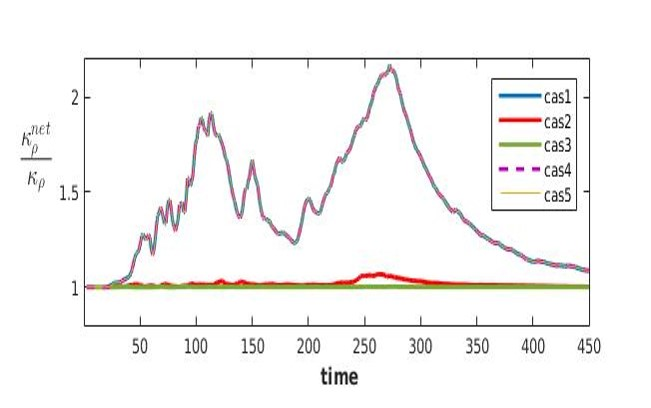
\includegraphics[width=0.9\linewidth]{figures/kappanet_rho.jpg}
        \caption{\textit{Évolution des diffusions nettes normalisées par la diffusion moléculaire explicite respective pour les cinq simulations}}
        \label{kappanet}
    \end{figure}


%----------------------------------------------------------------------------------
%%   RESULTATS
%----------------------------------------------------------------------------------
\newpage
\section{Résultats}

  \subsection{Variation du coefficient de diffuison de la densité}
  
    \subsubsection{Évolution de la densité et du traceur}

    \begin{figure}[!h]
    %\hfill
        \centering
        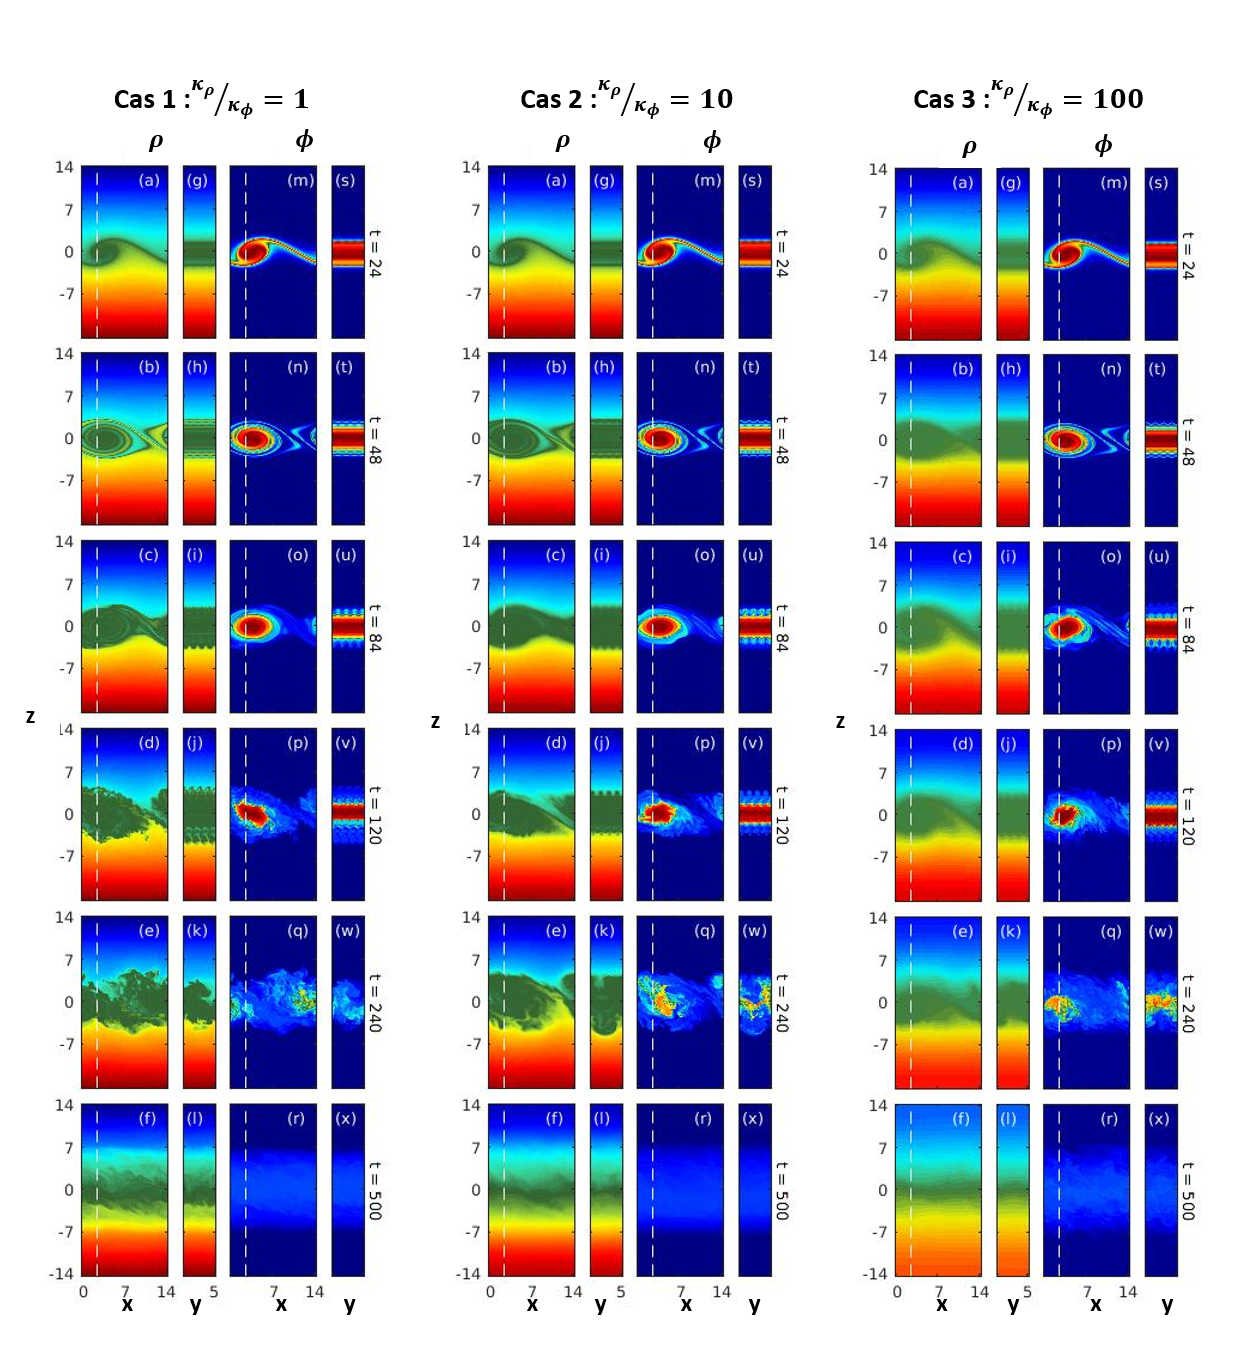
\includegraphics[width=0.95\linewidth]{figures/rhodiff_contour.png}
        \caption{\textit{Coupes z-x et z-y de la densité et du traceur passif des simulations 1, 2 et 3.}}
        \label{rhodiff}
    \end{figure}
    
    \begin{figure}[!h]
    %\hfill
        \centering
        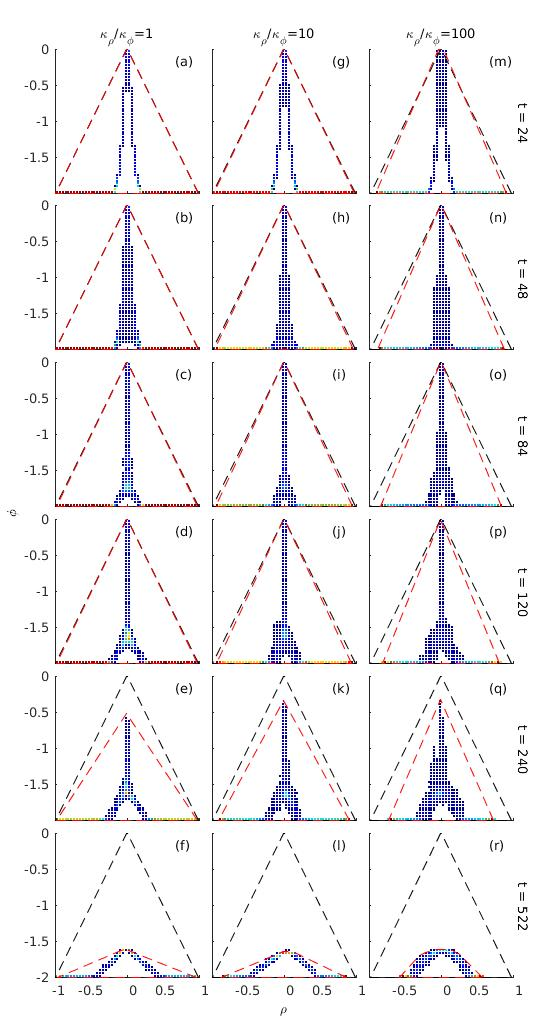
\includegraphics[width=0.6\linewidth]{figures/scatterplot_rhodiff.jpg}
        \caption{\textit{Diagrammes de dispersion aux mêmes pas de temps que la figure \ref{rhodiff} pour les simulations 1, 2 et 3.}}
        \label{scatterplot_rho}
    \end{figure}
    
    La figure \ref{rhodiff} présente des coupes z-x et z-y pour la simulation de références (cas 1) ou les coefficients de diffusion de la densité et du traceur sont les mêmes, et pour les simulations ou le coefficient de diffusion de la densité est 10 fois supérieur (cas 2), puis 100 fois supérieur (cas 3) à celui du traceur. À la première observation, même si l'évolution générale de la densité et du traceur semble proche, on voit que l'instabilité dynamique est modifiée avec le coefficient de diffusion de la densité. Les diagrammes de dispersion sont tracés sur la figure \ref{scatterplot_rho} aux mêmes pas de temps. 
    À t=24, le vortex typique des instabilités KH se forme. le diagramme de dispersion de la simulation de référence est proche de son état initial, ce qui veut dire que les particules sont seulement advectées de manière adiabatique (conservative) dans le vortex. Le pic correspond à la couche centrale de traceur, et sa largeur indique la pénétration du traceur dans les gammes de densités. Initialement, la majorité des particules fluides sont neutres en traceur, elles sont localisées à la base du diagramme de dispersion ($\phi=0$). Pour le cas 2 et 3 on note des signes de faible processus diabatique (non conservatif) liés à la diffusion lente de la densité, plus élevée dans ces deux simulations. 
    Le vortex continue d'étirer les surfaces isopycnales, ce qui favorise le mélange non conservatif en augmentant les gradients locaux. Sur les diagrammes de dispersion, on voit bien ce mélange diabatique à t=48 avec un étalement du nuage de point. 
    Quand les surface isopycnales sont trop étirées, des instabilités convectives déstabilisent le vortex (visible sur les coupes x-z de la figure \ref{rhodiff} à t=84). Comme la configuration est en 3D, des instabilités transverses se mettent également en place, on commence à les voir sur les coupes z-y. 
    À t=120, les instabilités transverses et convectives décomposent rapidement le vortex et favorisent une homogénéisation rapide en traceur et densité. 
    À t=240, les diagrammes de dispersion montrent que ce mélange turbulent réduit le pic lié à la couche centrale concentrée en traceur et donc favorisent une homogénéisation rapide des propriétés des particules fluides. On note aussi qu'un noyau central concentré en traceur s'est formé à la fois sur la figure \ref{rhodiff} et sur les diagrammes de dispersion. Le mélange non conservatif et la dissipation continuent de faire effet jusqu'à dissiper l'instabilité. Même si les étapes sont similaires pour les trois cas, les profils finaux sont différents à la fois sur les coupes verticales que sur les diagrammes de dispersion. Sur la figure \ref{rhodiff} le traceur semble s'homogénéiser moins bien pour le cas 3 alors que le gradient de densité sur tout le domaine est beaucoup plus faible, la couche centrale de densité n'est presque plus marquée. Pour les cas 1 et 2, la couche centrale s'est élargie verticalement en homogénéisant ses propriétés en densité et traceur. On note des différences sur les diagrammes de dispersion également. Pour le cas 1 on retrouve la forme linéaire par morceau décrite par \cite{penney_diapycnal_2020} avec du traceur dans des nouvelles gammes de densité. Pour le cas 2 le pic final semble légèrement dissymétrique. Enfin, pour le cas 3 on ne retrouve pas le même comportement, le nuage de point ne devient pas aussi compacte que pour les autres cas et un plateau s'est créé au sommet du pic alors qu'il semble moins étalé sur l'axe de la densité. Pour ce dernier cas, on a donc moins d'étalement du traceur dans des gammes de densité extrêmes, mais les particules affectées sont plus homogènes en concentration de traceur.
    
    \subsubsection{Évolution macroscopique}
    
    À partir des sorties des simulations précédentes, le profil macroscopique de la densité et du traceur passifs, issu de l'équation ???, sont calculés à chaque pas de temps (Figure \ref{rhodiff_star}). Pour les trois simulations, on retrouve les deux phases de mélange. La première à $t\approx50$ quand le vortex s'enroule, étire les surfaces isopycnales et augmente les gradients locaux, et à $t\approx250$ quand les instabilités transverses apparaissent. Pour la densité, dans les cas 1 et 2 (Figure \ref{rhodiff_star}a-b), ces deux évènements se traduisent par un étalement vertical de la couche centrale ($\rho\approx 0$), qui est de plus en plus marquée, alors que pour le cas 3(Figure \ref{rhodiff_star}c), les instabilités transverses semble faire disparaitre cette couche centrale. La couche centrale en traceur passif (Figure \ref{rhodiff_star}d-e-f) augmente progressivement pour les trois cas, mais le mélange homogénéise significativement la couche à partir de $t\approx 250$ dans les trois cas. 
    \\
    \begin{figure}[!h]
    %\hfill
        \centering
        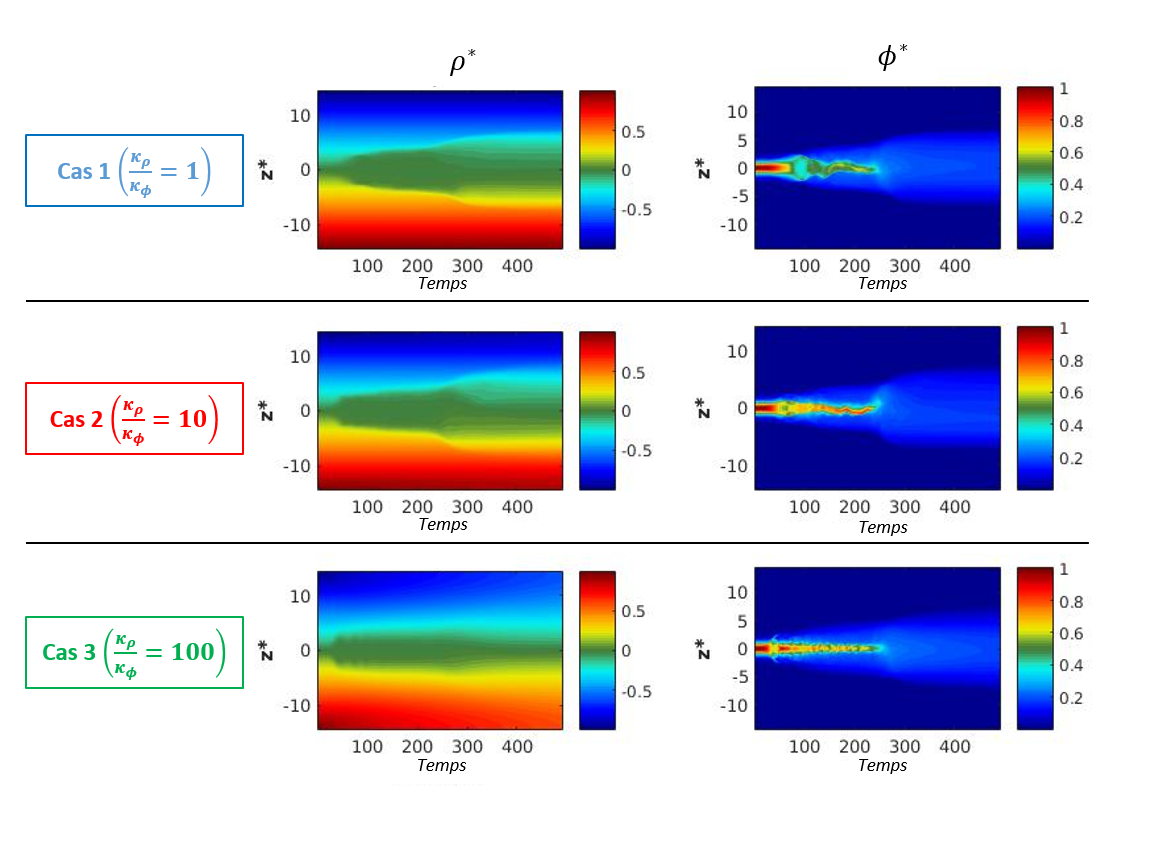
\includegraphics[width=0.9\linewidth]{figures/rhodiff_star.png}
        \caption{\textit{Évolution de $\rho_*$ et $\phi_*$ des simulations 1, 2 et 3.}}
        \label{rhodiff_star}
    \end{figure}
    Pour mieux analyser l'influence du mélange sur les profils macroscopiques, les profils finaux (t=500) issu du réarrangement sont tracés en trait plein sur la figure \ref{rhodiff_profils_Krho}. Sur cette figure, la densité a le même comportement que décrit précédemment. Pour le cas 1 et 2, elle a formé une couche centrale autour de $\rho\approx0$ alors que dans le cas 3 on ne distingue pas cette couche. Les interactions avec la surface et le fond modifient les profils finals avec l'augmentation du coefficient de diffusion (cas 2 et 3). Dans le cas 3 cette interaction est très marquée et pourrait donc avoir un impact sur la dynamique au centre de la colonne d'eau. Pour le traceur, on note un léger étalement vertical avec l'augmentation du coefficient de diffusion de la densité (cas 2 et 3).\\ 
    
    \begin{figure}[!h]
    %\hfill
        \centering
        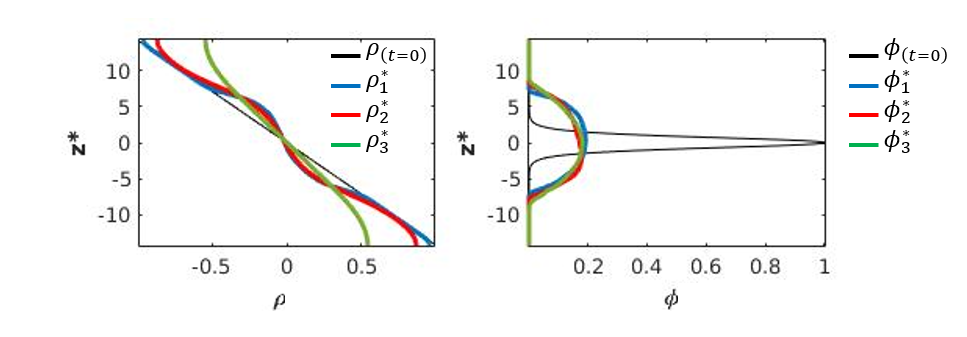
\includegraphics[width=1\linewidth]{figures/rhodiff_profils_fin.png}
        \caption{\textit{Profils verticaux finaux ($t=500$ de la densité (a) et du traceur passif (b) des simulations 1, 2 et 3.}}
        \label{rhodiff_profils_Krho}
    \end{figure}
    
    
  \subsection{Variation du coefficient de diffusion du traceur passif}
  
    \subsubsection{Évolution du traceur passif}
    
    \begin{figure}[!h]
    %\hfill
        \centering
        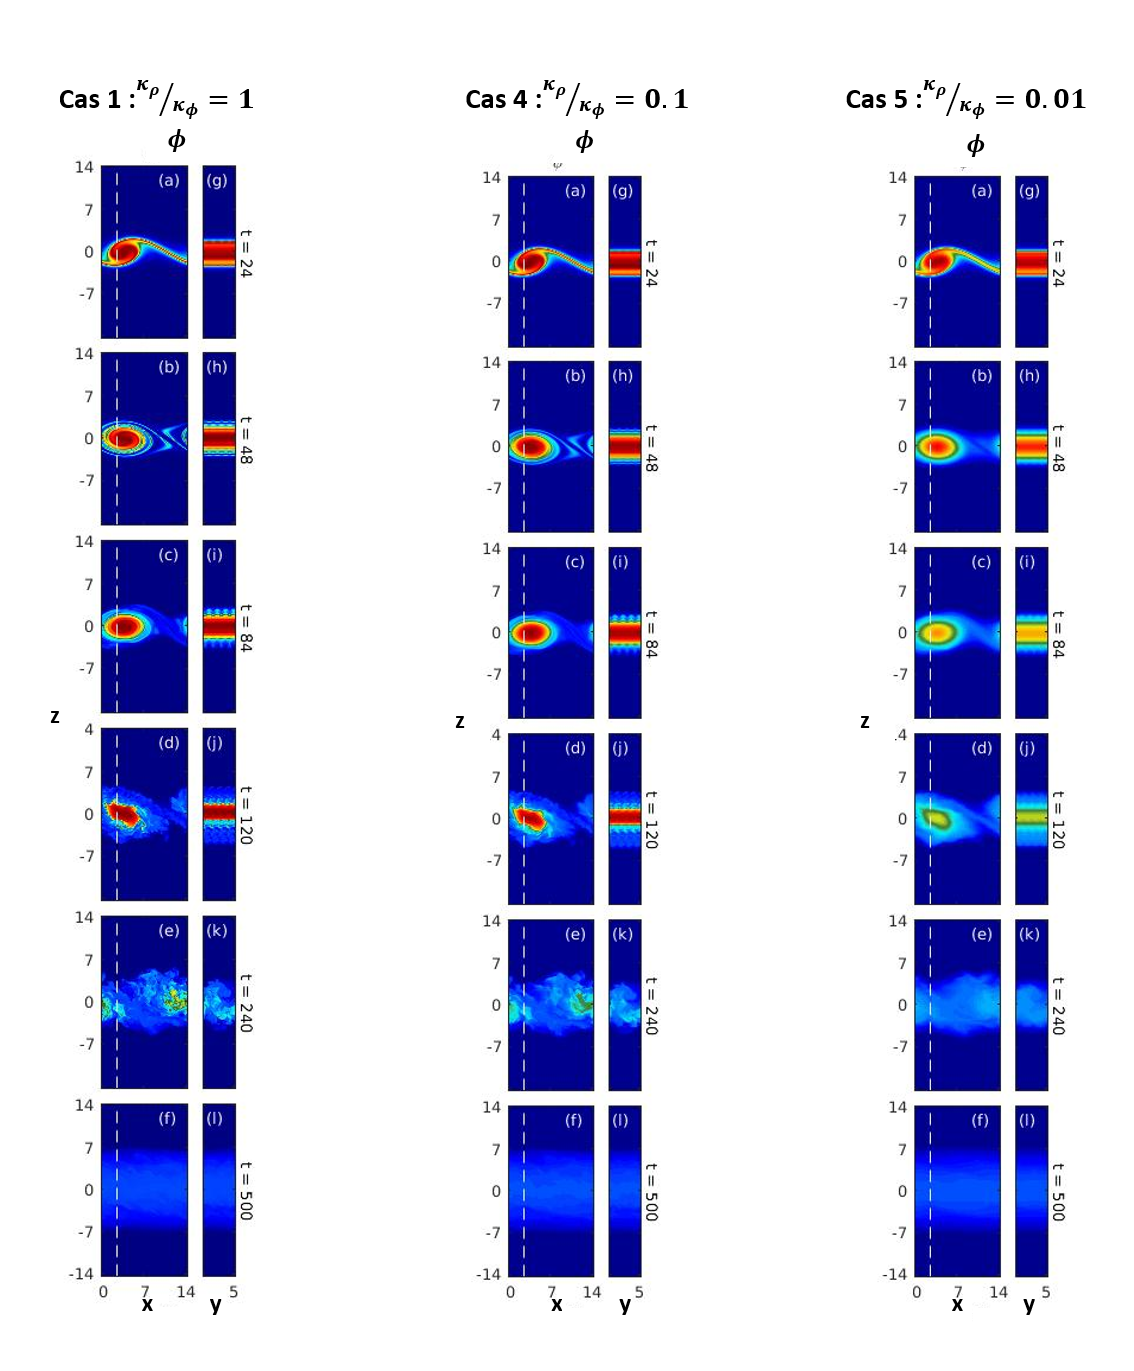
\includegraphics[width=0.90\linewidth]{figures/phidiff_contour.png}
        \caption{\textit{Coupes z-x et z-y du traceur passif des simulations 1, 4 et 5.}}
        \label{phidiff}
    \end{figure}
    
    \begin{figure}[!h]
    %\hfill
        \centering
        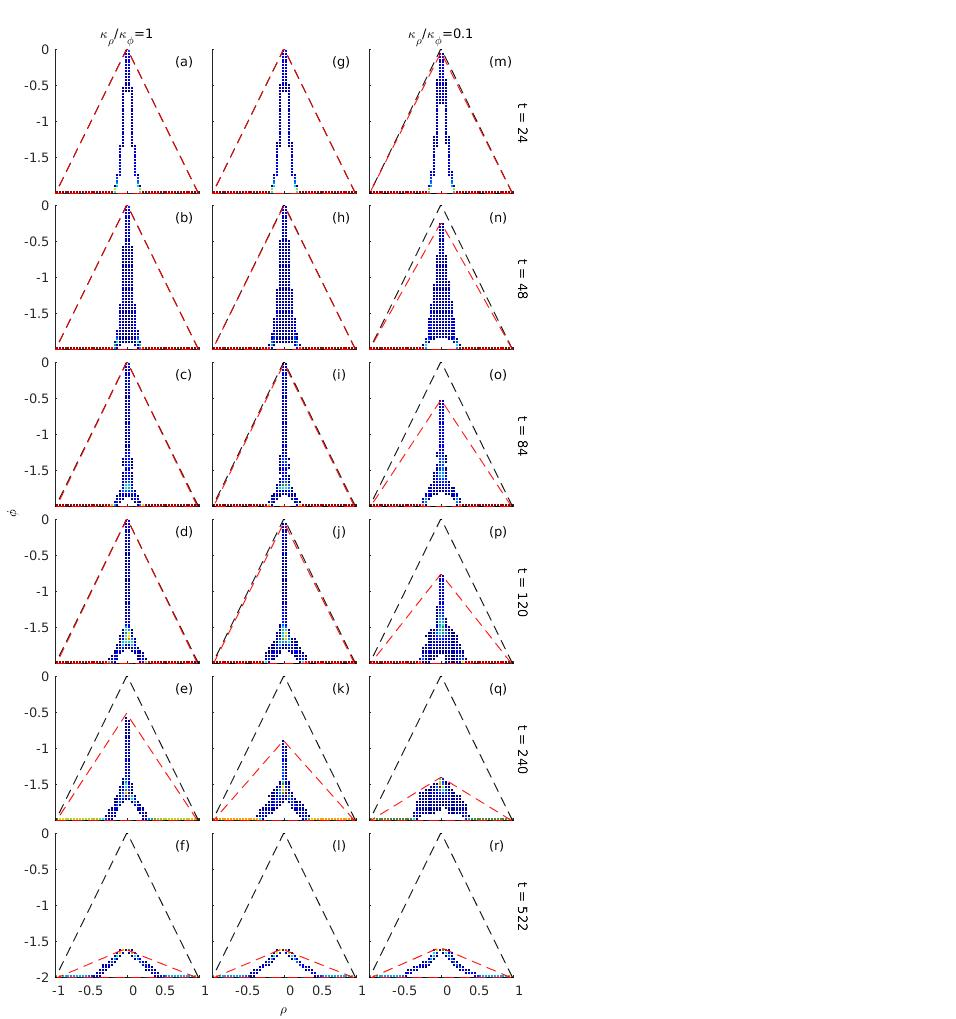
\includegraphics[width=0.7\linewidth]{figures/scatterplot_phidiff.jpg}
        \caption{\textit{Diagrammes de dispersion aux mêmes pas de temps que la figure \ref{phidiff} pour les simulations 1, 4 et 5.}}
        \label{scatterplot_phi}
    \end{figure}
    Dans cette parties les simulation 4 et 5 sont présentées. Elles correspondent respectivement à une multiplication du coefficient de diffusion moléculaire du traceur par 10 et par 100. Elles sont présentées avec le cas 1 qui est le cas de référence (même diffusion moléculaire pour le traceur et la densité).
    La variation du coefficient de diffusion du traceur n'affecte pas la dynamique, car le traceur est passif (il n'influe pas sur l'équation d'état). L'évolution de l'instabilité est donc la même que celle décrite pour le cas 1 dans la partie ???, c'est pourquoi seules les figures relatives au traceur passif sont présentées dans cette partie. Cependant, l'homogénéisation des particules en traceur est affectée, car on modifie le rayon d'action des particules fluides. Sur la figure \ref{phidiff} sont présentées les coupes verticales en traceur (x-z et y-z) pour les cas 1, 4 et 5, à plusieurs pas de temps. La diffusion lente est clairement visible pour le cas 5, mais les profils finaux semblent similaires dans les trois cas. Les diagrammes de dispersion correspondant aux mêmes pas de temps sont tracés sur la figure \ref{scatterplot_phi}. On note une diminution plus rapide du pic initial de la distribution avec l'augmentation du coefficient de diffusion du traceur passif, à partir de t=84 pour le cas 5 et t= 120 pour le cas 4, ce qui traduit un lissage des concentrations extrêmes en traceur plus efficace. La distribution finale du diagramme de dispersion du cas présente un profil linéaire par morceau comme attendu. Pour le cas 4 les segments semblent s'incurver de manière convexe, alors que pour le cas 5 les segments sont clairement incurvés et le sommet s'est arrondi.
    
    \subsubsection{Évolution macroscopique}
    
    \begin{figure}[!h]
    %\hfill
        \centering
        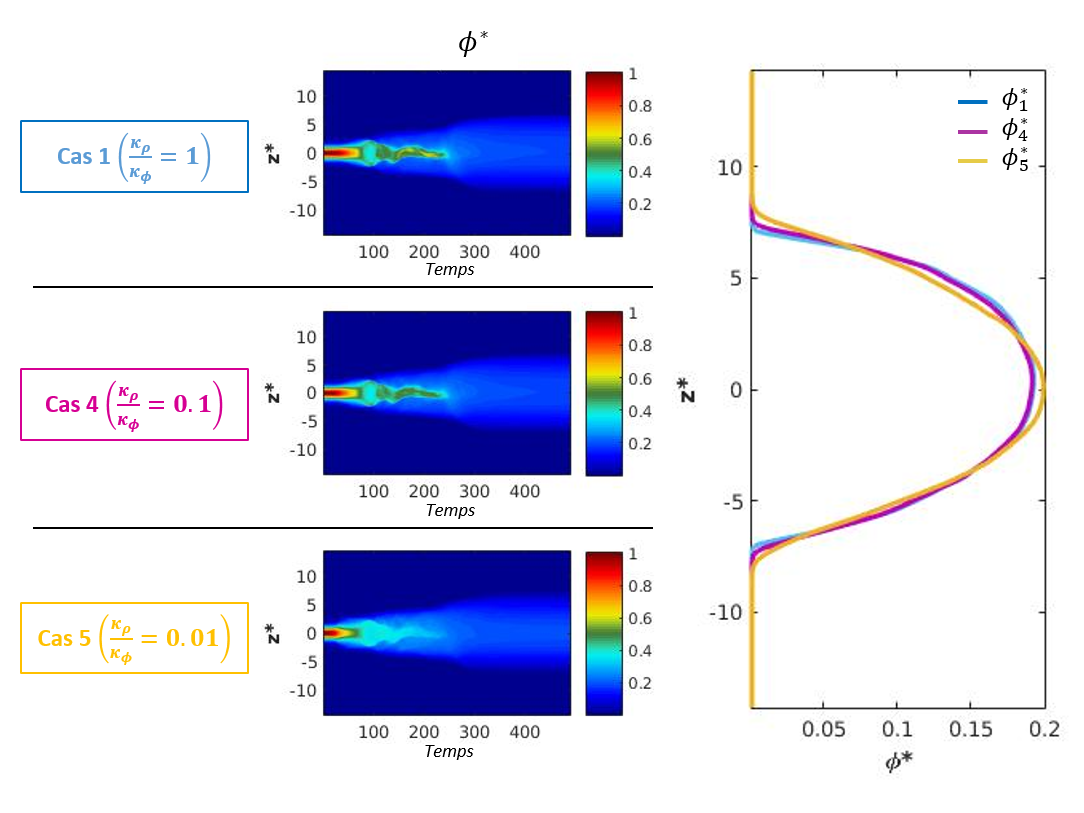
\includegraphics[width=1\linewidth]{figures/phidiff_star.png}
        \caption{\textit{(a) Évolution de $\rho_*$ et $\phi_*$ des simulations 1, 4 et 5. (b) Profils verticaux finaux ($t=500$) du traceur passif des simulations 1, 4 et 5.}}
        \label{phidiff_star}
    \end{figure}
    
    De la même manière que pour les 3 premières simulations, le profil macroscopique (réarrangement isopycnal) des traceurs a été calculé (Figure \ref{phidiff_star}). Il ne semble pas y avoir de grandes différences sur l'évolution du traceur passif entre les trois simulations, à partir de $t\approx250$ la couche de traceur s'homogénéise rapidement avec les instabilités transverses pour les trois simulations présentées ici. Cependant, quand on regarde le profil final (Figure \ref{phidiff_star}-b), on voit que le traceur pénètre dans des gammes de densité plus large avec un grand coefficient de diffusion (courbe violette et jaune).
    
  \subsection{Application de la diffusion effective $K_{\rho}^{eff}$ aux traceurs}
  
    \subsubsection{Application à la densité}
    \begin{figure}[!h]
        %\hfill
            \centering
            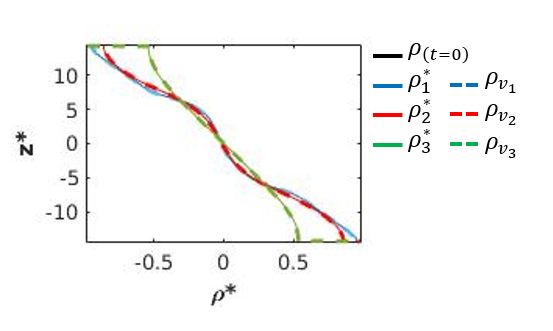
\includegraphics[width=0.5\linewidth]{figures/profils_Krho_rho.png}
            \caption{Figure à changer : split les trois profils sur trois figures (comme pour le traceur)}
            \label{profils_Krho_rho}
    \end{figure}
    
    Une équation de diffusion avec pour coefficient de diffusion $\K_\rho$ est appliquée au profil initial de densité. La variable obtenue est une densité virtuelle $\rho_v$ qui représente l'évolution d'un profil vertical macroscopique de la densité. D'après \cite{penney_diapycnal_2020} elle est supposée prédire l'évolution de la densité réarrangée $\rho_*$. Sur la figure \ref{profils_Krho_rho} le profil final (t=450) de $\rho_*$ est tracé en trait plein et celui de $\rho_v$ à t=450 est tracé en pointillé. Comme attendu, on retrouve exactement le même profil pour chaque simulation.
    
    \subsubsection{Application au traceur passif}
    
    De la même manière que pour la densité, une équation de diffusion avec pour coefficient $\frac{\kappa_{\phi}}{\kappa_{\rho}}$ est appliqué au profil initial du traceur pour chaque simulation. Les profils finaux de $\phi_*$ sont tracés en trait plein sur la figure \ref{profils_Krho} et les profils finaux de $\phi_v$ sont tracés sur la même figure en trait pointillé pour chaque cas. Comme attendu, pour le cas 1, le profil du traceur est prédit par le traceur virtuel. Ce résultat coïncide avec l'étude de \cite{penney_diapycnal_2020}. Pour les cas 2 et 3, quand la diffusion moléculaire de la densité est augmentée, le profil virtuel sous-estime la diffusion macroscopique du traceur alors que dans les cas 4 et 5, quand la diffusion moléculaire du traceur est augmentée, le profil virtuel sur-estime la diffusion macroscopique du traceur. 
    
    \begin{figure}[!h]
    %\hfill
        \centering
        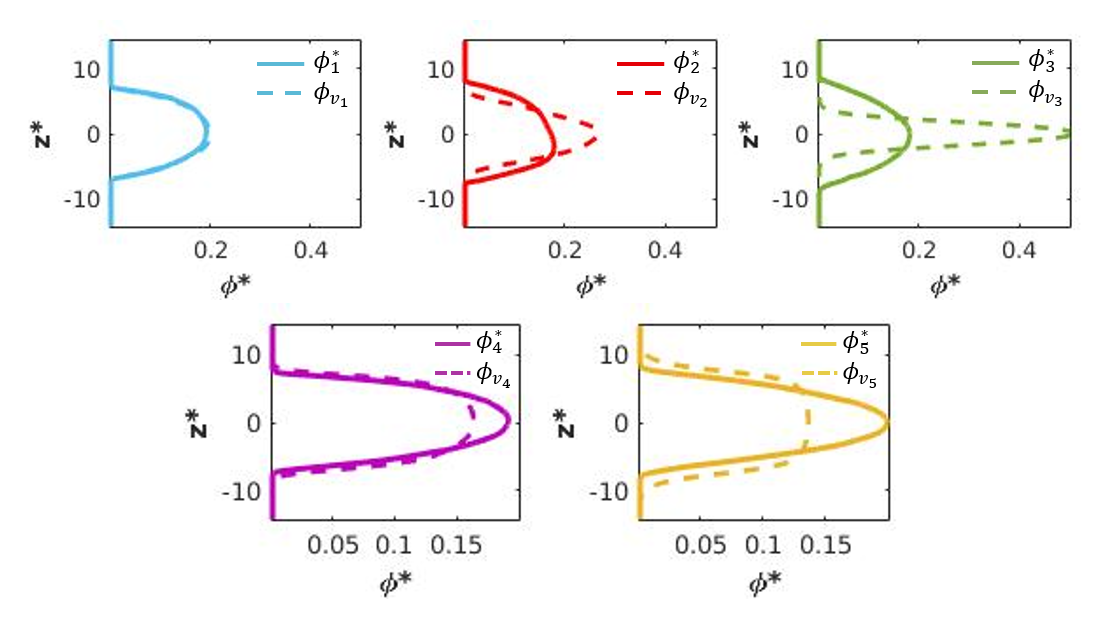
\includegraphics[width=1\linewidth]{figures/profils_Krho.png}
        \caption{\textit{Profils verticaux finaux (t=500) de $\rho_*$ et $\rho_v$ pour les cinq simulations.}}
        \label{profils_Krho}
    \end{figure}

%----------------------------------------------------------------------------------
%%   DISCUSSION
%----------------------------------------------------------------------------------

\section{Discussion}
    
    %\subsection{Stratification}
    Dans l'océan, la stratification est contrôlée à la fois par la température et la salinité. Ici une seule variable rentre dans l'équation d'état, donc pour se ramener à des cas réalistes, il faut considérer soit une stratification purement contrôlée par la température, soit une stratification purement contrôlée par la salinité. Cependant, la chaleur diffuse environ 100 fois plus que la salinité, donc le rapport avec la diffusion moléculaire des traceurs sera différent pour les deux cas. Les résultats ont montré l'importance de ce rapport et les différences de comportements quand $\kappa_{\rho}/\kappa_{\phi}$ est supérieur ou inférieur à 1 par rapport à la loi établi par \cite{penney_diapycnal_2020}. En effet, quand ce rapport est supérieur à 1, donc pour des grandes diffusions moléculaires de la densité, le mélange du traceur est clairement contrôlé par la dynamique. Or quand la densité diffuse beaucoup, elle a tendance à lisser l'instabilité et donc à agir comme un frein au mélange turbulent. Elle tend à retrouver une stratification linéaire (cas 3 de la figure \ref{rhodiff}-f-l). Sur les diagrammes de dispersion des cas 2 et 3, l'homogénéisation de la distribution met plus de temps à démarrer (figure \ref{scatterplot_rho} e-k-q). Quand le rapport des diffusions moléculaires est inférieur à 1, donc quand la diffusion du traceur est supérieur à celle de la densité, on distingue clairement deux phases. Le traceur lisse rapidement ses gradients, mais sans s'étaler dans de nouvelles gammes de densité. Ensuite, seule les processus de petites-échelles liés à la dynamique semble permettent un mélange plus efficace. Comme la dynamique finie par contrôler le mélange dans tous les cas, pendre en compte la viscosité dans les analyses devient important. Pour cette étude, la viscosité est restée fixe, mais on peut se demander comment le mélange serait affecté avec une viscosité plus élevée. En effet, la plus petite échelle contrôlant la dynamique, l'échelle de Kolmogorov, augmenterait et pourrait dépasser l'échelle de diffusion moléculaire. Dans ce cas, on s'attend à ce que le mélange soit moins efficace. En ce qui concerne la stratification, un cas n'est pas abordé ici. Le cas ou la stratification est à la fois contrôlé par la température et la salinité. Dans ce cas, les deux termes rentrent dans l'équation d'état de la densité. Celle-ci aura donc une diffusion qui dépend des deux variables, or, comme dit précédemment, la chaleur et la salinité ne diffusent pas à la même vitesse. Par exemple, dans l'océan, la fonte d'un iceberg en surface crée un apport d'eau douce froide, dans ce cas-là on parle de doubles diffusions. La stratification en température va entrainer une convection qui va elle-même créer une instabilité en sel. C'est une diffusion qui a déjà été étudié dans de nombreuses études (citer des articles ?) mais il serait intéressant de l'étudier avec l'approche présentée ici.
    \\
    %\subsection{Comportement à l'échelle macroscopique}
    \newline
    Les résultats présentés mettent en évidence une rupture comportementale à l'échelle macroscopique par rapport à la loi établie par \cite{penney_diapycnal_2020}. L'évolution du traceur ne peut plus être prédite à partir de la diffusion effective de la densité dès que les diffusions moléculaires entre traceur et densité sont différentes (figure \ref{profils_Krho}). C'est lié au fait que dans les cas 2, 3, 4 et 5, les diagrammes de dispersion ne convergent pas vers la même distribution que pour le cas 1. En effet, lorsque les diffusions moléculaires entre densité et traceur sont différentes, le rayon d'action de diffusion des particules fluides est différent dans l'espace traceur et dans l'espace densité. La convergence de la relation à l'échelle macroscopique ne peut donc pas se faire. Ce résultat met bien en évidence l'importance des processus petites-échelles sur les processus macroscopiques. Pour améliorer la paramétrisation des processus fine-échelles, il est donc nécessaire de mieux représenter l'évolution des traceurs passifs à l'échelle macroscopique. Une solution pourrait être de définir un coefficient de diffusion effectif pour chaque traceur en fonction de ses propriétés moléculaires. Cela impliquerait soit un développement complet de l'équation \ref{phi*} (évolution macroscopique du traceur) qui est plus complexe que l'équation macroscopique de la densité, soit de trouver des hypothèses simplificatrices, mais qui permettent quand même de représenter correctement les processus.
    \\
    %\subsection{Sensibilité à la configuration ?}
    \newline
    Dans cette étude, la position initiale du traceur est restée constante pour toutes les simulations. Cependant, dans la réalité, le traceur n'est pas toujours placé au centre de l'instabilité. \cite{penney_diapycnal_2020} ont montré que, pour des diffusions moléculaires égales, la position n'influençait pas le comportement des diagrammes de dispersion, et que le profil vertical final du traceur peut toujours être prédit par la diffusion effective de la densité. Donc, on ne s'attend pas à ce que la position affecte les tendances mises en évidence ici, mais il faudrait le vérifier. De plus, il faudrait vérifier la sensibilité au processus turbulent. Dans l'océan, la source de l'instabilité peut varier : cisaillement, convection, frottement de fond, tension du vent. Cependant, le principe de la cascade turbulente, donc de la descente vers les petites échelles, reste le même dans toutes les situations et dépend seulement des nombres sans dimension comme le nombre de Reynolds, de Richardson, de Prandtl ou de Schmitt. Donc, on ne s'attend pas à de que le processus turbulent ait beaucoup d'impact sur les résultats présentés ici.
    \\
    %\subsection{Aspects numériques}
    \newline
    Les éventuelles interactions avec la surface libre n'ont pas été étudiées afin de gagner en cout numérique. Mais la question de l'influence de la surface libre sur les processus turbulents est intéressante, car les couches de surface dans l'océan sont des couches de mélange. D'autant plus que la plupart des études sur les instabilités KH ne considèrent pas une surface libre dans leur simulation. Mais cela implique une augmentation de la vitesse acoustique afin de résoudre correctement les ondes de surface. Il faudrait donc mettre en place une nouvelle stratégie pour gagner en temps de calcul. L'équipe CROCO travail actuellement à déporter les calculs des CPU (processeurs) vers des GPU (cartes graphiques) plus efficace. Ils font un travail d'optimisation du code pour les GPU et établissent une communication avec les CPU qui s'occuperont toujours des sorties de simulations. 

%----------------------------------------------------------------------------------
%%   CONCLUSION
%----------------------------------------------------------------------------------

\section{Conclusion}


\newpage
\bibliographystyle{apalike}
\bibliography{bibstageM2}
%\bibliography{StageM2}
%citep %citet

\end{document}